

\begin{document}
This section details the calculations for the actively loaded MOSFET amplifier and the resistively loaded MOSFET amplifier. For the resistively loaded amplifier, calculations will be made to estimate appropriate resistor values for the circuit. Calculations will also be made for the various node voltages for each circuit

\subsection{Resistively loaded amplifier}

The resistively loaded differential amplifier uses two resistors attached to each drain of the amplifying N-channel MOSFETS (the ALD1006). The benefits of having a resistive load is the noise-reduction capabilities and faster switching due to lower capacitance of a given resistance. The disadvantage is that in order to attain higher gain, a larger drain resistor is required, which would negatively impact the operation of the amplifier if the size is too large. The differential voltage gain would be altered. The resistively loaded N-Channel MOSFET amplifier with a current mirror is shown in Figure \ref{fig:resistiveloadedgeneral}. 

\begin{figure}[H]
    \begin{center}
    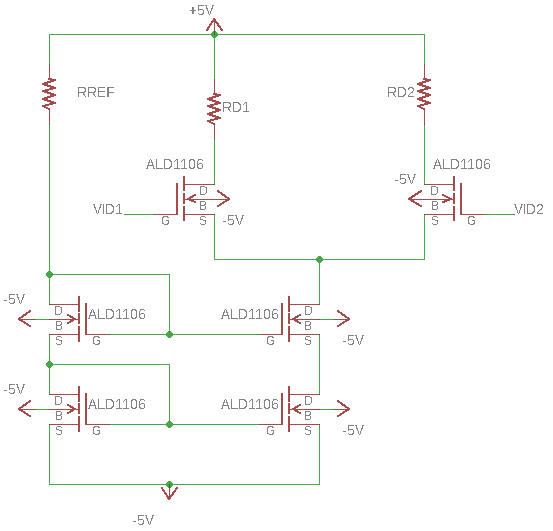
\includegraphics[scale=.85]{CircuitDevelopment/GenrealResLoaded.png}
    \caption{Resistively loaded differential amplifier}
    \label{fig:resistiveloadedgeneral}
    \end{center}
    
\end{figure}

The load resistors are RD1 and RD2. Their values need to be chosen to allow a bias current in each each resistor branch to equal $200\mu A$. Equation \ref{eqn:calc_RD} describes the calculation for both drain resistors.

\begin{equation}
    V_{o_1} = V_{DD} - \frac{1}{2}I_{bias}R_D\newline
     \label{eqn:calc_RD}
\end{equation}

Since the goal is to have the output voltages on in each branch to be equivalent at 2V, the equations can be solved for RD, which was found to be 15k$\Omega$. Now that the drain resistor values are calculated, the differential gain can be found using \ref{eqn:Ad_Res_Load}.

%differential gain equation

\begin{equation}
    A_d = \frac{1}{2}g_{m_N}(r_{o_N}//R_D) \approx \frac{1}{2} g_{m_N}R_D
     \label{eqn:Ad_Res_Load}
\end{equation}

Since $I_{bias} $ is $400\mu$ and both drain resistors are $15 k\Omega$, the differential gain was calculated at 3.18 $\frac{V}{V}$. The other value to be found is the single-ended common mode voltage gain, or $A_{cm}$. This is found using Equation \ref{eqn:Acm_Res_Load}.

\begin{equation}
    A_{cm} = \frac{R_D}{2R_{SS}}
    \label{eqn:Acm_Res_Load}
\end{equation}

The single ended common mode gain was found to be 0.903 $\frac{V}{V}$. Using the value found for the differential gain and the common mode gain, the common mode rejection ration is found suing Equation \ref{eqn:CMRR_Res_Load}

\begin{equation}
    CMRR = \mid\frac{A_d}{A_{cm}}\mid
    \label{eqn:CMRR_Res_Load}
\end{equation}

The common mode rejection ratio was calculated to be 3.5. This may be acceptable for the purposes of the lab, but a value this low may cause problems that arise from common mode signal inputs.

\subsection{Active Load Differential Amplifier}

Compared to the resistively loaded differential amplifier, the active load is preferred in many amplifier integrated circuits. The active load differential MOSFET amplifier has improved biasing and also has the capability of delivering a higher gain compared to to a drain-resistor implementation. The general schematic for the active load MOSFET differential amplifier is shown in Figure \ref{fig:activeloadedgeneral}.



\begin{figure}[H]
    \begin{center}
    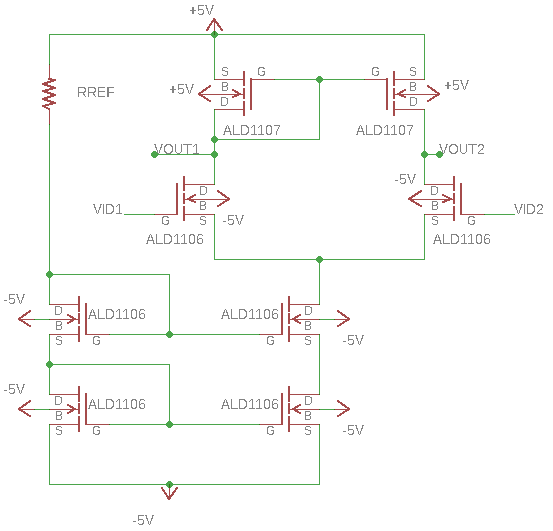
\includegraphics[scale=.85]{CircuitDevelopment/ActiveLoadedGeneral.png}
    \caption{Active load differential amplifier}
    \label{fig:activeloadedgeneral}
    \end{center}
    
\end{figure}

In place of the drain resistors in the previous circuit, two ALD1107 PMOS IC's are used in their stead, providing the active load. In order to calculate the double-ended gain, the inputs need to be grounded in the calculations. The differential gain is found using Equation \ref{eqn:Ad_Active_Load} below.

%differential gain equation
\begin{equation}
A_d = g_{m_P}(r_{o_P}//r_{o_N})
\label{eqn:Ad_Active_Load}
\end{equation}

The differential gain of the active load differential amplifier was calculated at 6.363 $\frac{V}{V}$. To calculate the value of the common mode gain, the thevenin equaivalent resistance of the current mirror, $R_{SS}$ needs to be found as well as the voltage at the input to the current mirror, $V_s$. This can be calculated by using Equation \ref{eqn:RSS_Active}

\begin{equation}
    R_{SS} = \frac{V_s-V_{SS}}{I_{bias}}
    \label{eqn:RSS_Active}
\end{equation}

The equivalent resistance was found to be 8.3$k\Omega$. This value is needed to find the common mode gain depicted in Equation \ref{eqn:Acm_Active_Load}.
%common mode gain equation
\begin{equation}
    A_{cm} = \frac{1}{2g_{m_N}R_{SS}}
    \label{eqn:Acm_Active_Load}
\end{equation}

The common mode gain was found to be 0.903 $\frac{V}{V}$. Using the common mode and differential gain found from Equation \ref{eqn:Ad_Active_Load} and Equation \ref{eqn:Acm_Active_Load}, the common mode rejection ratio can be found using Equation \ref{eqn:CMRR_Res_Load}. The CMRR was found to be 88.4 $\frac{V}{V}$. This value only denotes the double ended CMRR and gains. The single ended calculations result in a CMRR of 3.5. 



\end{document}